\documentclass[12pt]{article}
\usepackage{sbc-template}
\usepackage[T1]{fontenc}
\usepackage[utf8]{inputenc}
\usepackage[brazil]{babel}
\usepackage{graphicx,url,amsmath,amssymb,booktabs,tabularx,array}
\usepackage{hyperref}
\usepackage{tikz}
\usetikzlibrary{arrows.meta}
\hypersetup{hidelinks}
\sloppy
\title{RotasGraph: roteamento temporal e análise estrutural da rede de transporte público de Belo Horizonte}
\author{Caio Cesar Falinacio dos Santos\inst{1}, Gabriel Aredes\inst{1},\\
Joaquim Antonio\inst{1}, Luiz Fernando Cunha Maia\inst{1},\\
Pedro Henrique Nogueira\inst{1}, Wanessa Oliveira Marcos\inst{1}}
\address{Engenharia de Software -- Pontifícia Universidade Católica de Minas Gerais\\
(PUC Minas) -- Minas Gerais -- Brasil\\
Teoria dos Grafos e Computabilidade\\
Professor responsável: Leonardo Vilela Cardoso}
\newcommand{\code}[1]{\texttt{#1}}
\begin{document}
\maketitle
\begin{abstract}
RotasGraph computes earliest-arrival journeys from Belo Horizonte GTFS data using an in-memory directed temporal graph. A native Python A* combines timetable binary search with a Haversine lower bound. We state its correctness assumptions and account for ordered-list insertion and obsolete heap entries. Structural analysis of the selected service day finds 45 articulation points and 260 strongly connected components across 9,925 stops and 1,458,808 temporal connections. A REST interface geocodes addresses, attaches walking edges and displays public route numbers. Reproducible evidence and model limitations delimit the conclusions.
\end{abstract}
\begin{resumo}
O RotasGraph calcula trajetos de menor chegada a partir do GTFS de Belo Horizonte, em um grafo dirigido temporal mantido em memória. O A* em Python nativo combina busca binária de partidas e heurística de Haversine. Explicitamos as hipóteses de correção e os custos da inserção ordenada e das entradas obsoletas no heap. A análise do dia selecionado encontra 45 articulações e 260 componentes fortemente conexas em 9.925 paradas e 1.458.808 conexões temporais. A interface REST geocodifica endereços, acrescenta caminhadas e exibe números públicos de linhas. Evidências reproduzíveis e limitações delimitam as conclusões.
\end{resumo}

\section{Introdução}
O transporte público é uma aplicação de grafos em que conectividade e tempo não podem ser confundidos. A presença de uma linha entre duas paradas não significa que o passageiro possa utilizá-la no horário desejado. Uma conexão pode já ter partido, uma linha expressa pode sair depois e chegar antes, e uma viagem cadastrada pode operar somente em outro dia. Minimizar apenas a distância ou somar durações sem contabilizar esperas produz respostas incompatíveis com os horários publicados.

O objetivo deste trabalho é construir uma ferramenta para selecionar origem, destino e horário, calcular a menor chegada e apresentar um itinerário verificável. O recorte é Belo Horizonte, utilizando dados GTFS dos sistemas convencional e suplementar disponibilizados pela BHTRANS/SUMOB. O projeto também avalia cortes e componentes da malha, distinguindo resiliência estrutural de viabilidade temporal.

O núcleo mantém listas de adjacência na RAM e implementa os algoritmos com a biblioteca padrão de Python. Essa escolha atende ao objetivo disciplinar de demonstrar a construção, a correção e a complexidade do processamento de grafos. Bibliotecas prontas não substituem o motor: NetworkX é restrito à referência experimental. FastAPI expõe o domínio por HTTP, enquanto HTML, Tailwind compilado localmente e JavaScript nativo compõem a interface.

As contribuições são a integração de calendários e higienização GTFS a um grafo temporal, o A* com busca binária e prova condicional da heurística, a análise explícita dos custos reais das estruturas Python e uma análise estrutural independente da apresentação. Os resultados descrevem o feed selecionado e o ambiente observado; não constituem uma previsão de demanda, uma recomendação operacional à cidade ou uma prova de superioridade universal de um algoritmo.

\section{Problema, requisitos e recorte}
Uma consulta do motor é a tripla $(o,d,t_0)$, em que $o$ e $d$ são vértices distintos e $t_0$ é o horário inicial. No fluxo público, os endereços tornam-se vértices temporários ligados às paradas por caminhada. Minimiza-se $A(P,t_0)$ entre caminhos temporais viáveis; como $t_0$ é fixo, isso equivale a minimizar $A(P,t_0)-t_0$, incluindo caminhada, espera e transporte. Não se minimizam tarifa, distância, baldeações ou emissões.

A interface geocodifica endereços de Belo Horizonte. O passageiro confirma uma parada de origem dentro de seu limite; no destino, usa-se a mais próxima. Mudar endereço, parada ou limite invalida o resultado. A interface informa carregamento, ausência de rota e erros, e apresenta data de serviço, chegada, duração, espera, deslocamento, distância e instruções.

O dia de serviço é resolvido no servidor. Horários como \code{25:15:30} permanecem no serviço selecionado, sem módulo 24 ou busca automática no dia seguinte. O domínio não usa banco ou bibliotecas de grafos. Geoapify/OpenStreetMap fornecem apenas sugestões e coordenadas; roteamento e encaixe permanecem locais \cite{geocoding}. Entidades de alta cardinalidade usam \code{\_\_slots\_\_}.

O MVP admite transferência no mesmo instante e na mesma estação, sem penalidade mínima. Não modela lotação, atraso em tempo real, velocidade de ruas, acessibilidade física, regras tarifárias ou permanência no mesmo veículo. O resultado é ótimo para o modelo e os registros aceitos, não uma garantia sobre a operação observada nas ruas. Essa distinção é necessária para interpretar tanto a demonstração quanto os experimentos.

\section{Dados GTFS e construção da rede}
\subsection{Procedência e calendário}
O pacote oficial consultado em 17/11/2026 contém seis tabelas utilizadas: \code{stops.txt}, \code{routes.txt}, \code{trips.txt}, \code{stop\_times.txt}, \code{calendar.txt} e \code{calendar\_dates.txt} \cite{pbh}. O cadastro possui 9.925 paradas, 326 linhas, 113.692 viagens, 14 serviços e 67 exceções. Esses números descrevem o pacote, não as viagens ativas de uma consulta. A origem e os SHA-256 completos do ZIP e de cada CSV estão em \path{data/gtfs/README.md}.

A seleção semanal considera vigência inclusiva e dia da semana. Depois, exceções do tipo 1 adicionam serviços e do tipo 2 removem serviços para a data. Os calendários foram obtidos junto com os quatro arquivos principais, evitando misturar versões. A especificação GTFS descreve essa relação entre viagem, serviço e dia de operação \cite{gtfs}. Inferir o significado de um ID numérico, ou unir todos os serviços em uma única rede, permitiria combinar viagens que nunca operam juntas.

Para 17/11/2026, são selecionados \code{307679} e \code{307682}. A análise aprovada registra 25.956 viagens carregadas e 1.458.808 conexões, preservando todas as 9.925 paradas, inclusive as sem viagens ativas. O diagnóstico topológico registra 140 viagens rejeitadas. Registros de serviços inativos não são erros de CSV: são excluídos porque pertencem a outro calendário. O arquivo de horários ainda é lido integralmente, portanto filtrar o grafo reduz armazenamento, mas não elimina o custo de leitura do feed.

Os TXT são CSVs versionados por Git LFS. Um ponteiro LFS não é uma tabela e precisa ser substituído pelo objeto completo antes da carga. O controle de hashes identifica o conteúdo efetivamente processado; um novo download pode trazer outro feed na mesma URL. A validação local de dia útil, sábado e Carnaval está documentada, mas os resultados topológicos deste artigo correspondem exclusivamente a 17/11/2026.

\subsection{Higienização e perdas conservadoras}
O carregador valida cabeçalhos, coordenadas finitas, faixas geográficas, IDs e referências. Duplicatas idênticas preservam o primeiro cadastro; um mesmo ID com dados conflitantes é excluído. Os modais aceitos de linhas GTFS são 1 e 3, convertidos para \code{SUBWAY} e \code{BUS}. A disponibilidade desses tipos no domínio não comprova presença de ambos no feed de ônibus.

Os horários são processados por blocos contíguos de viagem e ordenados por \code{stop\_sequence} numérico. Uma viagem é validada integralmente antes da inserção: parada ausente, sequência repetida, duração negativa ou saída anterior à chegada rejeitam o bloco. Isso evita criar um atalho artificial ao simplesmente remover uma parada inválida do meio da viagem. Reaparição de uma viagem após outro bloco é falha estrutural explícita.

Tempo zero entre IDs diferentes coloca a viagem em quarentena. Restrições de embarque ou desembarque diferentes de zero também excluem a viagem inteira, pois \code{Connection} não mantém o estado de permanência no veículo. Para o dia analisado, o diagnóstico conta 2.106 registros por tempo zero e 3.034 por restrições, além de 5.201.100 registros de serviço inativo. Contagens de registros não equivalem a contagens de viagens.

Velocidade geodésica acima de 120 km/h é um alerta, não uma prova de erro nem um corte de velocidade. A distância é Haversine entre paradas, sem \code{shapes.txt} ou geometria de ruas. Os arquivos originais permanecem intactos: quarentena significa exclusão do grafo e registro de motivo, não edição do dataset. Assim, reexecutar a carga com a mesma versão e regras permite recuperar as decisões tomadas.

\section{Modelagem matemática e entidades}
O grafo é um multigrafo dirigido $G=(V,E)$: cada estação é um vértice e cada partida específica entre duas paradas consecutivas é uma aresta. Duas viagens da mesma linha em horários distintos geram conexões distintas, mesmo que possuam os mesmos extremos. Portanto, $E$ mede eventos temporais e pode ser muito maior que o número de pares adjacentes da malha.

Uma conexão armazena linha, destino, modal, distância, horário de partida $p_c$ e duração $\tau_c$. A origem é implícita na lista de adjacência. Para transporte agendado, a conexão só é utilizável quando $t\leq p_c$ e sua chegada é $a_c=p_c+\tau_c$. O custo é
\begin{equation}
w_c(t)=(p_c-t)+\tau_c=a_c-t,\qquad t\leq p_c.
\end{equation}
Conexões perdidas são indisponíveis. Para caminhada, a partida é imediata e o custo é $\tau_c$, com chegada $t+\tau_c$. O horário zero armazenado em uma aresta \code{WALK} é uma convenção interna e não significa que o passageiro deva partir à meia-noite.

\code{Station} usa \code{station\_id}; nomes iguais não colapsam paradas. \code{TemporaryVertex} representa os endereços. \code{Connection} conserva \code{route\_id} para o vínculo GTFS e \code{route\_short\_name} para apresentação. \code{TransportGraph} mantém listas ordenadas; \code{RouteSimulator} retorna caminho ou \code{None}; a API cria \code{Itinerary}. \code{TimeUtils} preserva horas estendidas.

\begin{figure}[ht]
\centering
\begin{tikzpicture}[
  box/.style={draw,rounded corners=1pt,align=left,text width=5.9cm,inner sep=6pt,font=\fontsize{10}{12}\selectfont},
  relation/.style={-{Latex[length=2mm]},line width=.5pt},
  relation label/.style={font=\fontsize{9}{11}\selectfont,fill=white,inner sep=2pt}
]
\node[box] (station) at (0,0) {\textbf{Station}\\\ttfamily station\_id, name\\latitude, longitude};
\node[box] (connection) at (7.7,0) {\textbf{\rmfamily Connection}\\\ttfamily route\_id, destination, vehicle\_type\\departure\_time, travel\_time, distance};
\node[box] (graph) at (0,-3.1) {\textbf{\rmfamily TransportGraph}\\\ttfamily add\_station(station)\\add\_connection(origin, connection)\\get\_neighbors(station)};
\node[box] (simulator) at (7.7,-3.1) {\textbf{\rmfamily RouteSimulator}\\\ttfamily calculate\_route(...)\\max\_speed\_of(graph)\\heuristic(current, target)};
\node[box] (loader) at (0,-6.2) {\textbf{\rmfamily DataLoader}\\\ttfamily build\_graph()\\\rmfamily Lê e higieniza o GTFS por data.};
\node[box] (itinerary) at (7.7,-6.2) {\textbf{\rmfamily Itinerary}\\\ttfamily steps, instructions, total\_seconds\\to\_dict(), to\_json()\\\rmfamily Criado pela API a partir do caminho.};
\draw[relation] (connection.west) -- node[relation label,above]{destino} (station.east);
\draw[relation] (graph.north) -- node[relation label,left]{vértices} (station.south);
\draw[relation] (graph.north east) -- node[relation label,sloped,above]{conexões} (connection.south west);
\draw[relation] (simulator.west) -- node[relation label,above]{consulta} (graph.east);
\draw[relation] (loader.north) -- node[relation label,left]{constrói} (graph.south);
\end{tikzpicture}

\caption{Visão resumida das entidades e contratos reais. A API cria o itinerário após receber o caminho; não há dependência do roteador para o itinerário. O diagrama completo permanece em \texttt{docs/diagrams/}.}
\label{fig:classes}
\end{figure}

O encaixe recebe coordenadas e limites independentes entre 100 m e 2 km. Percorre estações reais, calcula Haversine e ordena candidatas por distância e ID. A origem aceita qualquer candidata válida; o destino usa a primeira. Caminhadas adotam 5 km/h e arestas ponto--parada ou parada--ponto. Um \emph{overlay} privado evita mutar o grafo compartilhado e é limpo ao fim, inclusive sob exceção.

\section{A* dependente do tempo e correção}
\subsection{Rótulos, expansão e escolha de partidas}
O rótulo $g[v]$ representa a melhor chegada absoluta conhecida em $v$, com $g[o]=t_0$. O heap ordena por $f(v)=g[v]+h(v,d)$ e usa um contador para desempates, evitando comparar objetos \code{Station}. Cada relaxamento estritamente melhor atualiza o predecessor e insere nova entrada. Uma estação fechada não é expandida outra vez; entradas obsoletas permanecem no heap até sua remoção.

Ao expandir $v$ no instante $g[v]$, o algoritmo verifica o prefixo com horário zero para caminhadas. Em seguida, \code{bisect\_left} localiza a primeira conexão cuja partida não antecede $g[v]$. O sufixo viável é percorrido por índices, sem criar uma fatia de lista. A busca binária descarta partidas perdidas; não escolhe sozinha a melhor viagem.

Esse detalhe preserva correção quando uma partida posterior chega antes. Suponha duas ligações para o mesmo destino: saída às 08:00 com duração de 40 minutos e saída às 08:05 com duração de 10 minutos. Um passageiro presente às 07:59 deve escolher a chegada às 08:15. Examinar apenas a primeira partida aceitaria indevidamente 08:40. O roteador examina as duas e mantém o menor rótulo.

Se já há uma chegada conhecida $B$ no destino final, partidas $p_c\geq B$ podem encerrar a varredura ordenada. Durações e esperas não negativas implicam $a_c\geq p_c\geq B$, portanto nenhuma dessas conexões melhora a solução. Conexões anteriores ao limite continuam sendo avaliadas; a poda não substitui a comparação de chegadas.

\subsection{FIFO com possibilidade de espera}
Para um par de estações, defina a melhor chegada utilizável como o mínimo de $p_c+\tau_c$ sobre partidas $p_c\geq t$. Quando $t$ aumenta, o conjunto de opções só diminui, logo seu mínimo não diminui. Essa é a propriedade FIFO relevante ao modelo com espera. Ela não exige que todas as viagens sejam ordenadas por chegada na mesma ordem das partidas.

Chegar cedo a uma estação domina chegar tarde porque é permitido aguardar sem restrição. Assim, um rótulo de menor chegada conserva todas as escolhas disponíveis a um rótulo posterior. Caminhar imediatamente também satisfaz FIFO, já que $t+\tau_c$ é não decrescente. O argumento depende de não haver estado adicional, como veículo atual, limite de espera ou restrição de baldeação. Acrescentar esses requisitos exigiria rever os estados do grafo e a prova.

\subsection{Heurística consistente e admissível}
Usa-se $h(v,d)=d_H(v,d)/V_{\max}$, em que $d_H$ é Haversine e $V_{\max}$ limita superiormente a razão distância/duração de todas as conexões utilizáveis. O limite é derivado do grafo, e não do alerta de 120 km/h. Para qualquer conexão válida $(u,v)$, com distância igual à geodésica e duração positiva,
\begin{align}
d_H(u,d)&\leq d_H(u,v)+d_H(v,d),\\
d_H(u,v)/V_{\max}&\leq\tau_{uv}\leq w_{uv}(t).
\end{align}
Portanto, $h(u,d)\leq w_{uv}(t)+h(v,d)$ e $h(d,d)=0$. A heurística é consistente; somar a desigualdade ao longo de qualquer caminho viável prova sua admissibilidade. A espera aumenta o custo sem aumentar o limite inferior. Sob FIFO e consistência, retirar o destino como mínimo do heap encerra a busca com chegada ótima, conforme o princípio do A* \cite{hart}.

Uma velocidade máxima calculada ignorando durações não positivas não corrige uma aresta impossível. Por isso a carga exclui viagens com tempo zero entre estações distintas. Grafos construídos manualmente devem satisfazer as mesmas hipóteses. Um valor de velocidade excessivamente alto continua admissível, mas enfraquece a heurística; um valor baixo demais pode perder a garantia. Admissibilidade é propriedade do modelo e dos dados, não do nome do algoritmo.

\subsection{Reconstrução e apresentação do resultado}
O predecessor registra a conexão que melhorou cada estação. Ao alcançar o destino, o motor percorre esses vínculos e inverte a sequência. Sem caminho devolve \code{None}; origem igual ao destino devolve lista vazia internamente, embora o contrato HTTP rejeite essa consulta. Esses resultados não devem ser confundidos na interface.

\code{Itinerary} valida continuidade e horários, calcula espera e deslocamento e produz instruções em português. Horários absolutos são arredondados uma vez para segundos antes das diferenças, de modo que o total coincida com a soma dos trechos e com espera mais viagem. O A* mantém minutos fracionários durante toda a busca. A formatação não altera a escolha da rota e não inventa identificadores de viagem ausentes do domínio.

\section{Análise temporal e espacial}
Sejam $V$ o número de estações, $E$ o número de conexões temporais, $K_v$ a quantidade de saídas de $v$, $X$ o conjunto de estações expandidas, $H$ o número de inserções no heap, $L$ o número de trechos retornados e $C\leq V$ o número de candidatas de um encaixe. Operações em dicionários e conjuntos têm custo médio amortizado; os limites não pressupõem proteção contra colisões patológicas de hash. Campos de horários e IDs são considerados de tamanho limitado pelo feed analisado.

O grafo ocupa $O(V+E)$: há uma entrada por estação e uma referência por conexão. \code{\_\_slots\_\_} elimina o dicionário de atributos por instância e reduz constantes, mantendo a mesma ordem. Adicionar estação e recuperar a referência da adjacência custam $O(1)$ médio. Percorrer a lista retornada é outra operação e custa $O(K_v)$.

\code{add\_connection} encontra a posição por \code{bisect\_right}, mas \code{list.insert} pode deslocar $K_v$ referências \cite{python}. Assim, a inserção completa custa $O(K_v+1)$ no pior caso; quando ocorre no final, a mutação é $O(1)$ amortizado, porém a busca binária ainda custa $O(\log(K_v+1)+1)$. Não é correto chamar a inserção ordenada inteira de logarítmica. A construção incremental pode acumular $O(\sum_v K_v^2)$ em deslocamentos no pior caso, além do parsing e da ordenação interna das viagens.

Uma expansão custa $O(W_v+\log(K_v+1)+S_v+1)$, em que $W_v$ é o prefixo de horário zero e $S_v$ é o sufixo examinado. Logo, $O(\log K_v)$ descreve somente a localização da primeira partida. Como cada estação é expandida no máximo uma vez, as varreduras somam $O(E)$, e o custo refinado da consulta é
\begin{equation}
O\left(E+\sum_{v\in X}\log(K_v+1)+H\log(H+1)+L+|X|+1\right).
\end{equation}

O \code{heapq} não possui \emph{decrease-key}. Cada melhora insere uma tupla e conserva a entrada antiga, portanto $H=O(E+1)$ e o heap pode ocupar $O(E+1)$, não apenas $O(V)$. Definindo $K_{\max}=\max_v K_v$, com valor zero sem conexões, obtém-se
\begin{equation}
T_{A^*}=O\left(E\log(E+1)+V\log(K_{\max}+1)+L+V+1\right).
\end{equation}
Os termos constantes cobrem a inicialização e a expansão de uma origem isolada. O limite é rigoroso também quando $E=0$. A heurística pode reduzir trabalho observado, mas não melhora esse pior caso; uma heurística pouco informativa se aproxima de Dijkstra.

Rótulos, predecessores e fechados usam $O(V)$; o heap usa $O(E+1)$ e a reconstrução $O(L)$. O espaço auxiliar é $O(V+E)$. Em modo endereço, a aresta final exige ordenar uma adjacência adicional em $O(K_s\log(K_s+1))$, termo dominado por $O(E\log(E+1))$. O limite clássico com $\log V$ não vale automaticamente para este heap com duplicatas.

\begin{table}[ht]
\centering
\caption{Custos de apoio, além da consulta de menor chegada.}
\begin{tabularx}{\textwidth}{@{}lXX@{}}
\toprule Operação & Tempo & Espaço adicional \\
\midrule
Velocidade máxima & $O(V+E)$ & $O(1)$ \\
Heurística Haversine & $O(1)$ & $O(1)$ \\
Reconstrução / itinerário & $O(L)$ & $O(L)$ \\
Autocomplete geográfico & serviço externo; até 6 respostas & $O(1)$ com limite fixo \\
Candidatas do encaixe & $O(V+C\log(C+1))$ & $O(C)$ \\
Anexar / remover aresta temporária & $O(1)$ médio & $O(1)$ por ponta \\
Análise topológica & $O(V+E)$ esperado & $O(V+E)$ \\
\bottomrule
\end{tabularx}
\end{table}

\section{Análise estrutural e vulnerabilidade}
\code{GraphAnalyzer} ignora horários e durações e exclui vértices temporários. A análise de articulações usa uma projeção não direcionada simples: conexões paralelas tornam-se uma adjacência e autoarestas são ignoradas. Uma articulação é um vértice cuja remoção aumenta a quantidade de componentes conexas dessa projeção. Não se usa o termo para afirmar corte forte do grafo dirigido.

A busca em profundidade mantém descoberta e \emph{lowpoint}. Para um filho $v$ de $u$, a condição $low[v]\geq disc[u]$ identifica separação por $u$ não raiz; a raiz é articulação quando tem mais de um filho na árvore DFS. A implementação usa pilhas explícitas para não depender do limite de recursão do Python. A mesma travessia calcula o aumento de componentes após a remoção.

Para a rede dirigida, Tarjan iterativo mantém índices, valores baixos, pilha de vértices e pertencimento à pilha. Quando o índice de um vértice coincide com seu valor baixo, os vértices retirados até ele formam uma componente fortemente conexa (CFC) \cite{tarjan}. A projeção e as buscas custam $O(V+E)$ esperado; ordenar $C$ estações críticas acrescenta $O(C\log(C+1))$.

Define-se criticidade como $\max(0,\kappa(G-v)-\kappa(G))$, em que $\kappa$ conta componentes na projeção simples. O ranking usa score decrescente, depois grau simples decrescente e ID crescente. Ele mede fragmentação adicional, não passageiros afetados, centralidade de demanda ou perda de cobertura geográfica. Grau de estação não é quantidade de partidas porque arestas paralelas foram deduplicadas.

\begin{table}[ht]
\centering
\caption{Topologia de 17/11/2026. Fonte: \texttt{docs/analysis/topology.json}.}
\label{tab:topology}
\begin{tabular}{@{}lr@{}}
\toprule Indicador & Valor \\
\midrule
Estações reais registradas & 9.925 \\
Conexões temporais aceitas & 1.458.808 \\
Viagens carregadas & 25.956 \\
Pontos de articulação na projeção & 45 \\
Componentes fortemente conexas & 260 \\
Estações na maior CFC & 9.665 \\
Estações na segunda CFC & 2 \\
CFCs unitárias & 258 \\
\bottomrule
\end{tabular}
\end{table}

As CFCs totalizam 9.925 estações: $9.665+2+258$. A maior contém aproximadamente 97,38\% do cadastro. As componentes unitárias não devem ser rotuladas todas como paradas isoladas: um vértice pode ter conexões de entrada ou saída e ainda não participar de um ciclo dirigido. A Tabela~\ref{tab:topology} descreve conectividade estrutural; mesmo dois vértices na maior CFC podem não ter viagem viável a partir de um horário específico.

\begin{table}[ht]
\centering
\caption{Cinco primeiras estações do ranking estrutural aprovado.}
\begin{tabularx}{\textwidth}{@{}lXr@{}}
\toprule ID & Nome no feed & Score \\
\midrule
14784866 & Rod Anel Rodoviario Celso Mello Azevedo 22499 & 2 \\
14785457 & Avenida Presidente Antonio Carlos 3721 & 1 \\
14792434 & Pca Engenheiro Flavio Gutierrez 1 & 1 \\
14785996 & Rua Professor Eduardo Afonso De Morais 410 & 1 \\
14789634 & Rua Jeronimo Firmino Martins 131 & 1 \\
\bottomrule
\end{tabularx}
\end{table}

O primeiro score indica duas componentes adicionais após a remoção dessa parada, em relação ao número anterior. Não significa duas linhas interrompidas. O JSON guarda os 45 IDs de articulação, todos os tamanhos de CFC, até vinte posições do ranking e hashes de origem. As regras de higienização e a manutenção de estações sem serviço alteram a projeção; repetir a análise para outra data exige reconstruir o grafo e registrar nova procedência.

\section{Arquitetura, API e interface}
A inicialização do FastAPI carrega uma rede para \code{GTFS\_SERVICE\_DATE} e mantém grafo, índice de estações, data e velocidade máxima compartilhados. Cada busca cria seu simulador e seu overlay temporário, sem reingestão ou mutação das conexões comuns. Sem data configurada, a interface estática e \code{/health} respondem, mas consultas de rede retornam 503. O endpoint de saúde comprova disponibilidade da aplicação, não a existência de uma rede carregada.

\begin{figure}[ht]
\centering
\begin{tikzpicture}[
  layer/.style={draw,rounded corners=1pt,align=center,text width=12.9cm,inner sep=6pt,font=\fontsize{10}{12}\selectfont},
  tool/.style={layer,text width=5.9cm},
  relation/.style={-{Latex[length=2mm]},line width=.5pt},
  relation label/.style={font=\fontsize{9}{11}\selectfont,fill=white,inner sep=2pt}
]
\node[layer] (frontend) at (0,0) {\textbf{Frontend}\\HTML, Tailwind local e JavaScript nativo; mapa SVG e timeline};
\node[layer] (api) at (0,-1.9) {\textbf{FastAPI}\\\texttt{GET /stations} e \texttt{POST /routes/search}\\RouteNetwork compartilha grafo, índice, velocidade e data de serviço.};
\node[layer] (domain) at (0,-4.1) {\textbf{Domínio em memória}\\TransportGraph + RouteSimulator (A* temporal)\\Itinerary (passos, totais e instruções) + TimeUtils};
\node[tool] (loader) at (-3.5,-6.5) {\textbf{Ingestão}\\DataLoader + calendário\\Seis TXT GTFS locais via Git LFS};
\node[tool] (cli) at (3.5,-6.5) {\textbf{Ferramentas de linha de comando}\\Validação, benchmark e GraphAnalyzer\\Relatórios JSON e CSV};
\draw[relation] (frontend.south) -- node[relation label,right]{HTTP / JSON} (api.north);
\draw[relation] (api.south) -- node[relation label,right]{consulta e criação do itinerário} (domain.north);
\draw[relation] (loader.north) -- node[relation label,above right]{constrói o grafo} (domain.south west);
\draw[relation] (cli.north) -- node[relation label,above left]{consulta e analisa} (domain.south east);
\draw[relation] (cli.west) -- node[relation label,above]{usa} (loader.east);
\end{tikzpicture}

\caption{Visão resumida dos componentes implementados. As setas indicam comunicação ou uso; a API carrega a rede via DataLoader na inicialização. As ferramentas analíticas são executadas por linha de comando.}
\label{fig:components}
\end{figure}

\code{GET /stations} preserva a busca por parada. \code{POST /snap/candidates} lista paradas entre 100 m e 2 km. \code{POST /routes/search} aceita o modo por IDs ou \code{address}, com coordenadas, limites e parada de origem; a partida usa \code{HH:MM}. \code{/config/geocoding} informa a disponibilidade do autocomplete. Combinações incompletas são rejeitadas.

Um caminho retorna 200 com \code{status=found}; ausência usa \code{status=no-route}. ID desconhecido ou nenhuma parada no limite gera 404; coordenadas, limites ou origem inválidos geram 422; rede indisponível gera 503. A API cria \code{Itinerary} sem recalcular a rota. A análise topológica continua na linha de comando.

O adaptador frontend concentra Fetch e conversões. O Geoapify restringe resultados a Belo Horizonte, exige três caracteres e retorna até seis endereços; chamadas antigas são canceladas. A origem recomenda a parada mais próxima, mas aceita outra candidata válida. O modal de caminhada ajusta cada ponta por metro; o destino é automático. Mudanças cancelam a rota anterior e o formulário bloqueia envio duplicado.

O mapa projeta cada trecho: ônibus vermelho, metrô azul e caminhada cinza tracejada. Endereços, paradas e marcadores A/B compartilham a transformação; o desenho é esquemático e seu viewport se expande quando necessário. A timeline preserva horários e mostra \code{route\_short\_name}, nunca \code{route\_id}; sem nome público, usa ``Linha não informada''.

\begin{center}\begin{minipage}{.80\textwidth}
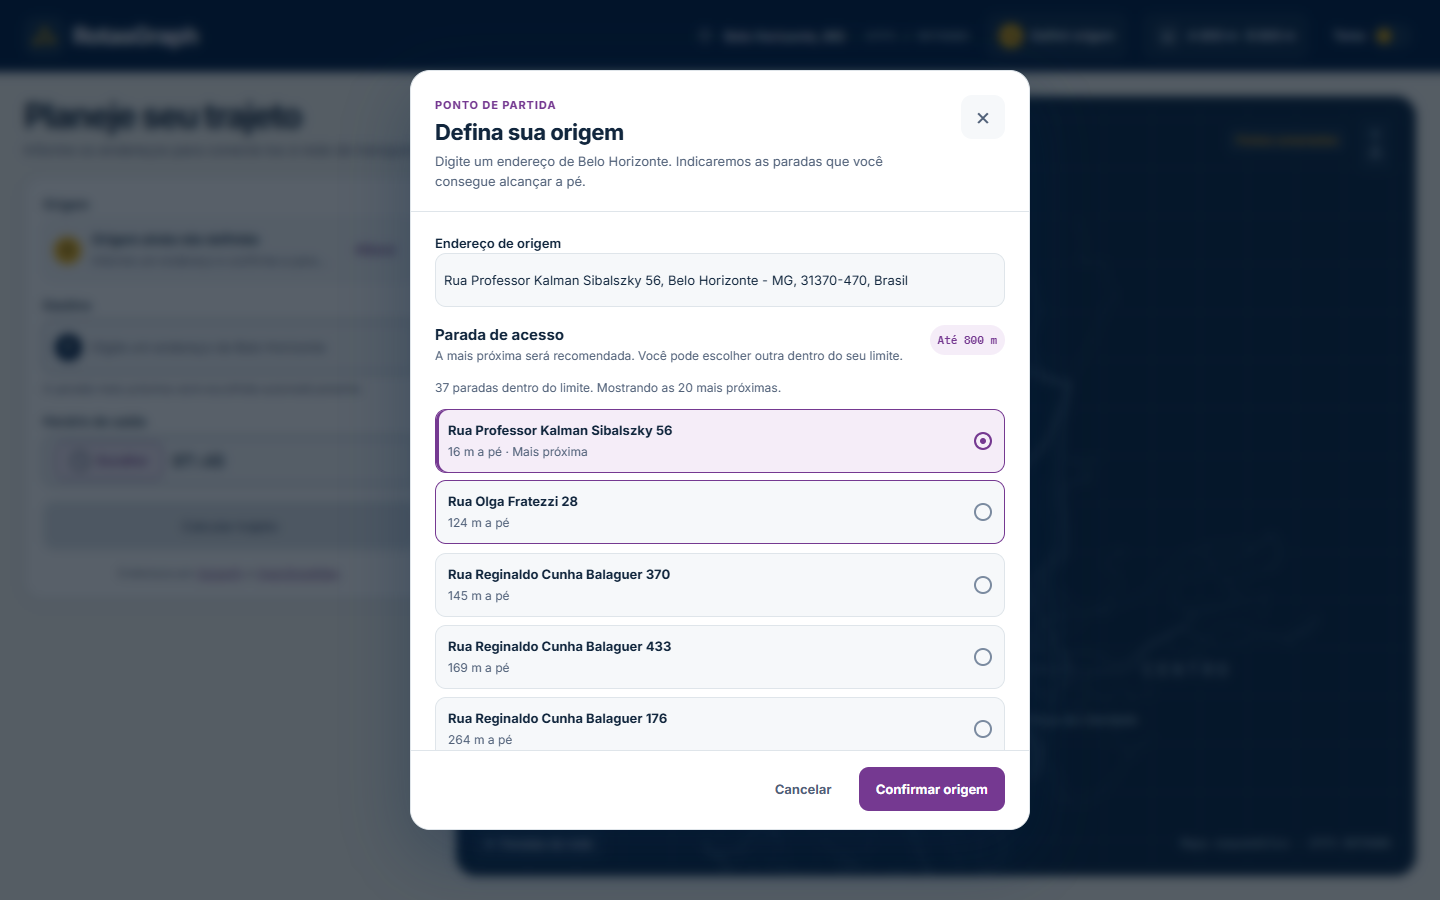
\includegraphics[width=\linewidth]{figures/interface-origin-snap.png}
\captionof{figure}{O endereço de origem é convertido em coordenadas; a parada mais próxima é recomendada e outras candidatas dentro do limite continuam disponíveis.}
\label{fig:search}
\end{minipage}\end{center}

\begin{center}\begin{minipage}{.80\textwidth}
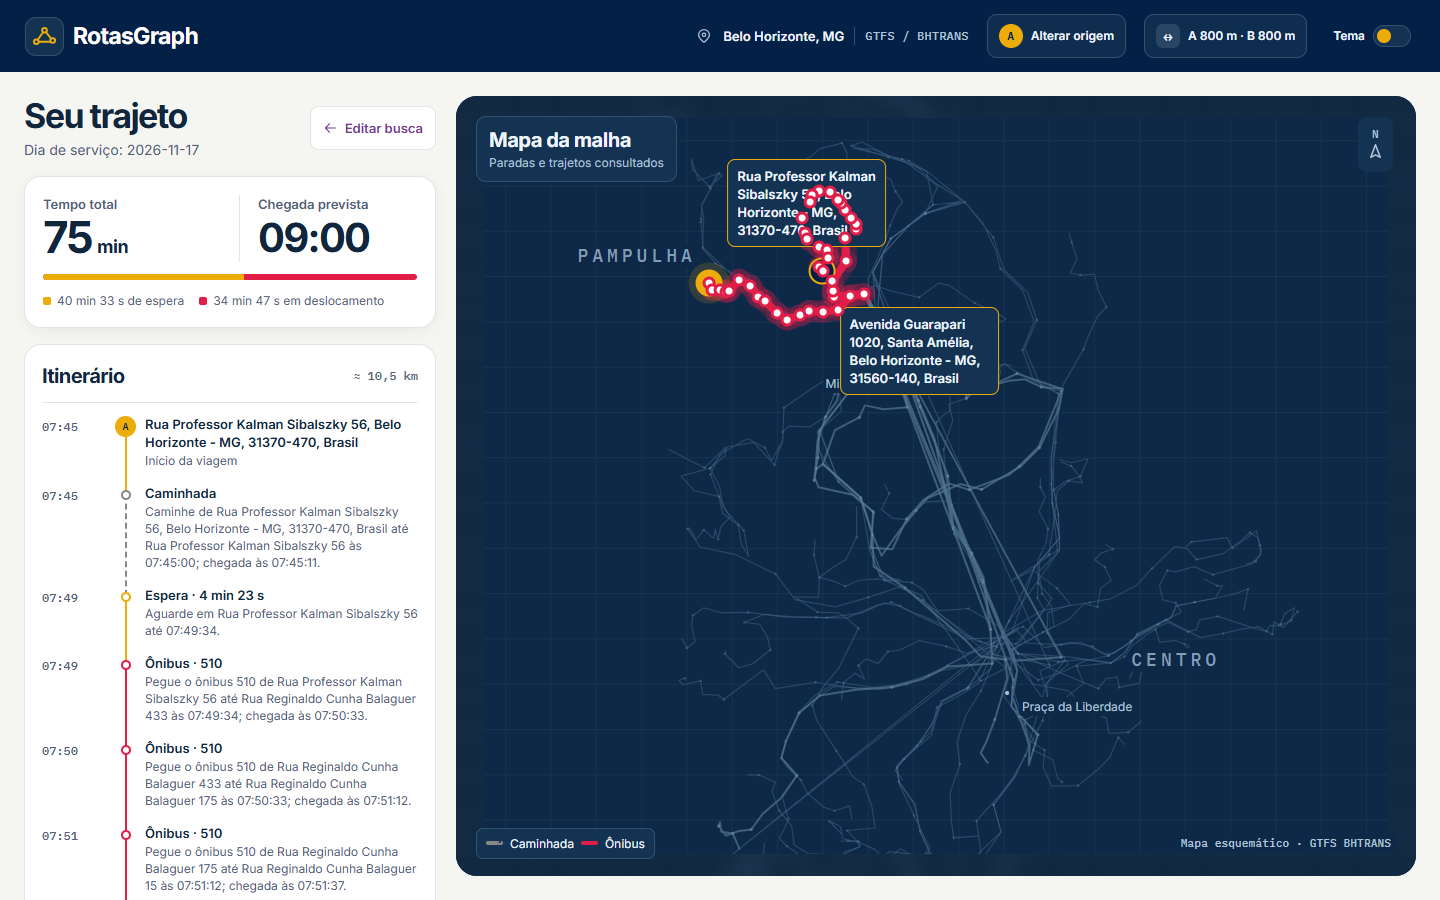
\includegraphics[width=\linewidth]{figures/interface-result.png}
\captionof{figure}{Resultado real por endereços: caminhada de acesso, número público da linha, espera, mapa e timeline derivados da mesma resposta da API.}
\label{fig:result}
\end{minipage}\end{center}

As capturas documentam o fluxo integrado. Da Rua Professor Kalman Sibalszky 56 à Avenida Guarapari 1020, às 07:45 de 17/11/2026, há caminhadas de 16 m e 30 m. A chegada ocorre às 09:00:20, com 40 min 33 s de espera e 34 min 47 s em deslocamento. A timeline mostra 510; o ID interno 561865 permanece apenas no GTFS.

\section{Verificação e avaliação experimental}
Os testes do motor usam grafos sintéticos para isolar o comportamento e não depender de download LFS. Incluem partida exata, conexão perdida, espera, baldeações, destino inalcançável, caminhada, reconstrução e uma partida posterior que chega antes. A comparação com Dijkstra dependente do tempo em grafos pequenos verifica a chegada ótima e a continuidade temporal do caminho. Concordância em uma amostra é evidência de regressão, não substitui as hipóteses da prova.

A ingestão cobre calendários, exceções, duplicidades, coordenadas, referências, sequências, nomes públicos e quarentena. O analisador cobre cadeia, ciclo, componentes, paralelas, autoarestas e vazio. A API testa candidatos ordenados, limites por metro, coordenadas inválidas, estação fora do raio, caminhada nas duas pontas, limpeza do overlay e rede indisponível.

Na integração visual, verificam-se desktop, celular, temas, movimento reduzido, teclado, edição e cancelamento. Testes isolam horário, modais, endereço, Geoapify, limites e número público da linha. O fluxo das Figuras~\ref{fig:search} e~\ref{fig:result} foi refeito em 1440 por 900 pixels. Testes DOM não equivalem a certificação integral de acessibilidade.

O benchmark compara o A* nativo com Dijkstra do NetworkX em uma expansão temporal equivalente. Cada evento de estação e horário torna-se um vértice; arestas de viagem e espera conservam a semântica temporal. O grafo de referência é uma representação diferente, portanto comparar somente o laço de busca esconderia custos de adaptação e preparação. Medem-se separadamente preparação, busca e consulta completa, com verificação de chegada ou ausência de caminho \cite{networkx}.

O manifesto seleciona oito pares distintos com semente 42: distâncias Haversine curtas abaixo de 2 km, médias entre 2 e menos de 8 km e longas a partir de 8 km, em 07:00 e 14:00, além de dois casos sem rota. A seleção preenche estratos usando a rede completa e registra sua procedência. Os casos sem rota encontrados são das 07:00. Essa amostra deliberada serve à caracterização, não estima a distribuição de viagens da população.

A campanha usa redes com 100, 1.000 e todas as estações, dois aquecimentos e sete repetições, com limite por processo de 600 segundos e RSS amostrada de 4.096 MiB. A execução de 21/11/2026 usou Windows 11, Python 3.14.7, NetworkX 3.7 e psutil 7.2.2, sobre a revisão \code{b4359d6} com alterações locais. Metadados, hashes e amostras estão em \path{docs/benchmarks/campaign/}. O IQR é calculado com quantis inclusivos; não se confunde com a diferença entre a menor e a maior mediana de casos distintos.

\subsection{Resultados e interpretação}
A matriz terminou válida, sem timeout, excesso de RSS ou divergência: são 54 processos, 384 amostras e 96 resumos. Os subgrafos preservaram os extremos das consultas, mas 100 estações produziram zero conexões e 1.000 produziram 15.722; nenhum dos oito pares teve rota nesses recortes. Essas latências medem respostas sem rota, não escalabilidade de itinerários alcançáveis. Na rede completa, com 9.925 estações e 1.458.808 conexões, a referência expandida tem 1.479.535 eventos e 2.926.010 arestas. Seis casos têm rota e dois não; ambos os motores concordam em chegada ou ausência de caminho.

\begin{table}[ht]
\centering
\caption{Custo completo da consulta na rede completa, em ms: mediana e IQR de sete repetições. Fonte: \texttt{campaign/full/summary.csv}.}
\label{tab:query-benchmark}
\begin{tabular}{@{}lrrrr@{}}
\toprule
& \multicolumn{2}{c}{A* nativo} & \multicolumn{2}{c}{Dijkstra NetworkX} \\
Caso & Mediana & IQR & Mediana & IQR \\
\midrule
long-07 & 1.640,334 & 219,319 & 113,803 & 6,619 \\
long-14 & 1.111,706 & 193,058 & 195,255 & 55,802 \\
medium-07 & 410,340 & 16,342 & 27,856 & 1,661 \\
medium-14 & 264,174 & 22,199 & 17,620 & 0,352 \\
short-07 & 149,375 & 21,296 & 4,286 & 1,012 \\
short-14 & 67,510 & 3,410 & 4,438 & 1,787 \\
no-route-1 & 2.595,359 & 258,083 & 8.290,382 & 1.873,659 \\
no-route-2 & 188,883 & 4,128 & 146,531 & 5,250 \\
\bottomrule
\end{tabular}
\end{table}

A Tabela~\ref{tab:query-benchmark} inclui preparação e limpeza específicas de cada consulta, além da busca, sem repetir a preparação global da rede. NetworkX apresenta menor mediana nos seis casos alcançáveis; o caso \code{no-route-1} inverte essa relação e é o mais lento em ambos. Distância Haversine caracteriza os estratos, mas não isola a dificuldade de busca. Os valores não autorizam combinar casos em um ganho universal.

\begin{table}[ht]
\centering
\caption{Preparação e RSS: \texttt{campaign/full/results.json}.}
\label{tab:prepared-benchmark}
\begin{tabular}{@{}lrr@{}}
\toprule Medida & A* nativo & Dijkstra NetworkX \\
\midrule
Preparação mediana (ms) & 734,682 & 14.333,139 \\
RSS preparada mediana (MiB) & 212,301 & 2.237,703 \\
Pico máximo amostrado (MiB) & 228,215 & 2.488,203 \\
\bottomrule
\end{tabular}
\end{table}

A preparação é a mediana entre nove processos por motor e inclui a importação fria de NetworkX. A RSS preparada é um snapshot do Python após a preparação; o pico é o máximo amostrado entre processos, somando raiz e descendentes uma vez por PID. Inclui ingestão, launcher, conversão e serialização, pode perder picos breves e não mede memória física exclusiva. Não se subtraem picos para obter memória da busca.

O monitor consulta a árvore de processos aproximadamente a cada 10 ms e pode interferir no tempo; não houve controle pareado desse efeito. As medianas da ingestão comum foram 96,434 s nos processos nativos e 33,818 s nos de NetworkX, evidenciando condições de execução diferentes. Os extremos foram preservados. Preparação, consultas amortizadas e RSS descrevem esta campanha e representações diferentes, sem estabelecer superioridade geral.


\section{Limitações e ameaças à validade}
A validade interna depende da equivalência temporal entre o motor e a referência, da seleção de serviços correta e da verificação de caminhos. Um teste que consultasse um grafo com calendários misturados poderia concordar matematicamente e ainda representar um dia impossível. Da mesma forma, um benchmark sobre um subgrafo não substitui medições da rede completa: remoção de estações modifica alcançabilidade e quantidade de conexões examinadas.

O modelo mantém uma única melhor chegada por estação porque a espera é permitida e não há estado de veículo ou tarifa. Uma extensão com tempo mínimo de transferência, continuidade a bordo ou restrições de embarque exigiria estados adicionais ou nova política de relaxamento. A quarentena atual evita trajetos sabidamente incompatíveis com esse domínio, ao custo de excluir serviços potencialmente utilizáveis em uma modelagem mais rica.

Haversine mede linha reta, não distância viária ou rota caminhável; o raio pode atravessar barreiras físicas e o mapa é apenas esquemático. O ótimo usa horários planejados, sem tarifa, lotação, acessibilidade de calçadas, trânsito ou cancelamentos ao vivo. O autocomplete depende da disponibilidade, cota e precisão do Geoapify/OpenStreetMap; o texto sai do navegador, mas não é persistido. A chave pública deve ser restrita por referenciador. O provedor não recebe o grafo nem calcula a rota.

A validade externa é limitada a um feed, um dia de serviço e um ambiente computacional. CPU, memória, sistema operacional, versão do interpretador e atividade concorrente afetam tempos e RSS. Aquecimentos e repetições reduzem ruído, mas não tornam oito pares uma amostra representativa. Uma implementação pode vencer em busca e perder no custo total de preparação; nenhuma conclusão geral deve ignorar essa separação.

A análise de articulação é não direcionada e sem tempo. O ranking não estima número de passageiros, frequência de atendimento ou importância socioeconômica. A maior CFC demonstra caminhos dirigidos estruturais, sem assegurar compatibilidade de horários. Articulações e CFCs ajudam a discutir fragilidade matemática da rede aceita, mas não bastam para decidir alterações de infraestrutura.

\section{Reprodutibilidade e responsabilidades}
As entradas e evidências permanecem separadas: \path{data/gtfs/README.md} identifica o feed; \path{docs/analysis/topology.json} contém resultados topológicos; \path{docs/benchmarks/} contém manifestos e relatórios experimentais. Diagramas editáveis Mermaid e seus PNG/SVG ficam em \path{docs/diagrams/}, incluindo casos de uso, classes, componentes, estados e duas sequências. As fontes deste artigo e da apresentação permitem recompilar os PDFs, usando o estilo SBC de dezembro de 2017 \cite{sbc}, cuja origem e licença são registradas em \path{docs/report/TEMPLATE_SOURCE.md}.

Execute \code{git lfs pull} e \code{git lfs fsck}; validação e topologia usam \code{--date 2026-11-17}. O autocomplete requer \code{GEOAPIFY\_API\_KEY} em \path{.env.local}, nunca no artigo. Rode \code{python -m pytest} em \path{backend/} e \code{npm test}, \code{npm run build} e \code{npm run check:server} em \path{frontend/}; o último exige a aplicação ativa.

O histórico auditado é o conjunto alcançável por \code{HEAD} na revisão \code{b4359d6}, com 116 commits: 110 sem merge e seis merges. Os aliases são consolidados pelo e-mail do autor, sem reescrever histórico. A Tabela~\ref{tab:authors} resume responsabilidades sustentadas por commits, e \path{docs/AUTHORSHIP_AUDIT.md} apresenta contagens, e-mails, método e evidências individuais. Quantidade de commits não mede esforço ou qualidade.

\begin{table}[ht]
\centering
\caption{Responsabilidades comprovadas pelo histórico integrado.}
\label{tab:authors}
\begin{tabularx}{\textwidth}{@{}p{.34\textwidth}X@{}}
\toprule Integrante & Contribuições documentadas \\
\midrule
Caio Cesar Falinacio dos Santos & Planejamento, slots, A* temporal, velocidade máxima e testes com oráculo. \\
Gabriel Aredes & Conversões temporais, interface responsiva, seleção e verificação estática. \\
Joaquim Antonio & Dataset, carregador e calendários GTFS, itinerário e benchmark inicial. \\
Luiz Fernando Cunha Maia & Grafo ordenado, pontos temporários, higienização, integração e mapa. \\
Pedro Henrique Nogueira & Entidades e ciclo de vida da rede, endpoints de estações e rotas. \\
Wanessa Oliveira Marcos & Testes iniciais, endpoint de saúde, Haversine e heurística. \\
\bottomrule
\end{tabularx}
\end{table}

Os módulos foram modificados por mais de uma pessoa ao longo do desenvolvimento. Contribuições da consolidação ainda não commitadas, incluindo a auditoria e os artefatos acadêmicos, não recebem autoria individual inferida. A explicação oral é distribuída conforme as áreas registradas. O roteiro de 15 minutos está em \path{docs/VIDEO_SCRIPT.md}; gravação, participação dos seis membros e envio da entrega permanecem atividades humanas.

\section{Conclusão}
O RotasGraph integra GTFS, grafo em memória, A* temporal e trajetos entre endereços. O snap acrescenta caminhadas sem mutar a rede; a tela separa número público e ID interno. Sob FIFO e heurística consistente, obtém-se a menor chegada. A análise inclui varredura após bisect, inserção ordenada, candidatas e duplicatas no heap.

A rede de 17/11/2026 apresenta 45 articulações e 260 CFCs, sem inferência sobre demanda. A campanha confirmou equivalência nos oito casos completos, com seis alcançáveis. Preparação e RSS menores no motor nativo coexistem com consultas de comportamento diferente por caso. Representações, amortização e condições da máquina impedem declarar superioridade geral de A* ou Dijkstra.

Estado de viagem, transferências mínimas, geometria viária e múltiplos dias são extensões possíveis. Cada uma exige rever estados, dominância dos rótulos e validação, mantendo explícitos o modelo e seus limites.

\small
\begin{thebibliography}{99}
\setlength{\itemsep}{0pt}
\bibitem[Hart et al. 1968]{hart} Hart, P. E., Nilsson, N. J. e Raphael, B. (1968). A formal basis for the heuristic determination of minimum cost paths. \emph{IEEE Transactions on Systems Science and Cybernetics}, 4(2), 100--107. \url{https://doi.org/10.1109/TSSC.1968.300136}.
\bibitem[Tarjan 1972]{tarjan} Tarjan, R. (1972). Depth-first search and linear graph algorithms. \emph{SIAM Journal on Computing}, 1(2), 146--160. \url{https://doi.org/10.1137/0201010}.
\bibitem[MobilityData 2026]{gtfs} MobilityData. \emph{GTFS Schedule Reference}. \href{https://gtfs.org/documentation/schedule/reference/}{Documentação oficial}. Consulta em 21/11/2026.
\bibitem[PBH 2026]{pbh} Prefeitura de Belo Horizonte. \emph{Dados abertos: GTFS}. \href{https://ckan.pbh.gov.br/dataset/gtfs}{Portal oficial}. Pacote consultado em 17/11/2026.
\bibitem[Python Software Foundation 2026]{python} Python Software Foundation. \emph{bisect} e \emph{heapq}. \href{https://docs.python.org/3/library/}{Biblioteca padrão}. Consulta em 21/11/2026.
\bibitem[NetworkX 2026]{networkx} NetworkX Developers. \emph{single\_source\_dijkstra}. \href{https://networkx.org/documentation/stable/reference/algorithms/generated/networkx.algorithms.shortest_paths.weighted.single_source_dijkstra.html}{Documentação oficial}. Consulta em 21/11/2026.
\bibitem[Geoapify/OSM 2026]{geocoding} Geoapify. \href{https://apidocs.geoapify.com/docs/geocoding/address-autocomplete/}{Address Autocomplete API}. OpenStreetMap contributors. \href{https://www.openstreetmap.org/copyright}{Copyright and License}. Consulta em 22/11/2026.
\bibitem[SBC 2017]{sbc} Sociedade Brasileira de Computação. \href{https://www.overleaf.com/latex/templates/sbc-conferences-template/blbxwjwzdngr}{SBC Conferences Template}, dezembro de 2017. Licença CC BY 4.0.
\end{thebibliography}
\end{document}
